\begin{figure} [H]
    \begin{center}
        \tikzset{every picture/.style={line width=0.75pt}} %set default line width to 0.75pt        
        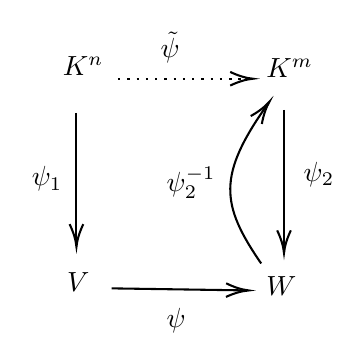
\begin{tikzpicture}[x=0.75pt,y=0.75pt,yscale=-1,xscale=1]
            %uncomment if require: \path (0,300); %set diagram left start at 0, and has height of 300

            %Straight Lines [id:da695871819745131] 
            \draw    (128,101) -- (128,163.5) ;
            \draw [shift={(128,165.5)}, rotate = 270] [color={rgb, 255:red, 0; green, 0; blue, 0 }  ][line width=0.75]    (10.93,-3.29) .. controls (6.95,-1.4) and (3.31,-0.3) .. (0,0) .. controls (3.31,0.3) and (6.95,1.4) .. (10.93,3.29)   ;
            %Straight Lines [id:da656763463540512] 
            \draw    (145,185.5) -- (209,186.47) ;
            \draw [shift={(211,186.5)}, rotate = 180.87] [color={rgb, 255:red, 0; green, 0; blue, 0 }  ][line width=0.75]    (10.93,-3.29) .. controls (6.95,-1.4) and (3.31,-0.3) .. (0,0) .. controls (3.31,0.3) and (6.95,1.4) .. (10.93,3.29)   ;
            %Straight Lines [id:da46225545196828643] 
            \draw    (228,99.5) -- (228,166.5) ;
            \draw [shift={(228,168.5)}, rotate = 270] [color={rgb, 255:red, 0; green, 0; blue, 0 }  ][line width=0.75]    (10.93,-3.29) .. controls (6.95,-1.4) and (3.31,-0.3) .. (0,0) .. controls (3.31,0.3) and (6.95,1.4) .. (10.93,3.29)   ;
            %Straight Lines [id:da17654653607895265] 
            \draw  [dash pattern={on 0.84pt off 2.51pt}]  (148,84.5) -- (211,84.5) ;
            \draw [shift={(213,84.5)}, rotate = 180] [color={rgb, 255:red, 0; green, 0; blue, 0 }  ][line width=0.75]    (10.93,-3.29) .. controls (6.95,-1.4) and (3.31,-0.3) .. (0,0) .. controls (3.31,0.3) and (6.95,1.4) .. (10.93,3.29)   ;
            %Curve Lines [id:da8908595252766036] 
            \draw    (217,173.5) .. controls (197.3,144.93) and (196.03,130.92) .. (219.89,97.06) ;
            \draw [shift={(221,95.5)}, rotate = 125.54] [color={rgb, 255:red, 0; green, 0; blue, 0 }  ][line width=0.75]    (10.93,-3.29) .. controls (6.95,-1.4) and (3.31,-0.3) .. (0,0) .. controls (3.31,0.3) and (6.95,1.4) .. (10.93,3.29)   ;

            % Text Node
            \draw (120,72.4) node [anchor=north west][inner sep=0.75pt]    {$\mathbb{K}^{n}$};
            % Text Node
            \draw (122,176.4) node [anchor=north west][inner sep=0.75pt]    {$V$};
            % Text Node
            \draw (218,178.4) node [anchor=north west][inner sep=0.75pt]    {$W$};
            % Text Node
            \draw (218,73.4) node [anchor=north west][inner sep=0.75pt]    {$\mathbb{K}^{m}$};
            % Text Node
            \draw (105,125.4) node [anchor=north west][inner sep=0.75pt]    {$\psi_1 $};
            % Text Node
            \draw (236,123.4) node [anchor=north west][inner sep=0.75pt]    {$\psi_2 $};
            % Text Node
            \draw (170,193.4) node [anchor=north west][inner sep=0.75pt]    {$\psi $};
            % Text Node
            \draw (167,60.4) node [anchor=north west][inner sep=0.75pt]    {$\tilde{\psi} $};
            % Text Node
            \draw (170,125.4) node [anchor=north west][inner sep=0.75pt]    {$\psi^{-1}_2 $};
        \end{tikzpicture}
    \end{center}
\end{figure}



